The goal of this chapter is to give a detailed description of the \textit{Bacco} protocol and to discuss the
implementation choices that were taken in order to deploy it. This is achieved using a top-down ordering for the level
of detail, meaning that an overview of the network is to be presented before going into the specifics.

\section{Overview}
The network is built upon 3 fundamental categories of devices:

\begin{description}[font=$\bullet$~\normalfont\scshape\color{blue!50!black}]
    \item [Sender node] - collects data and sends it to the gateway using LoRa
    \item [Repeater node] - listens to the incoming LoRa messages and repeates them
    \item [Gateway node] - collects data coming from the sender nodes and sends it to the web server using the FTP
        protocol over a mobile network such as \gls{GSM} or \gls{LTE} \footnote{A gateway can be configured to optionally perform
        pre-processing operations (e.g.\ filtering, smoothing, interpolation ...) of the incoming data and can
        even collect relevant data on-site when needed}. This node has also the role to coordinate the sender nodes that are
        sending data to it
    \item [Web server] - receives data coming from the gateways through FTP, elaborates it and makes it available to
        consult through a self-hosted web application platform
\end{description}

\begin{figure}[ht]
    \centering
    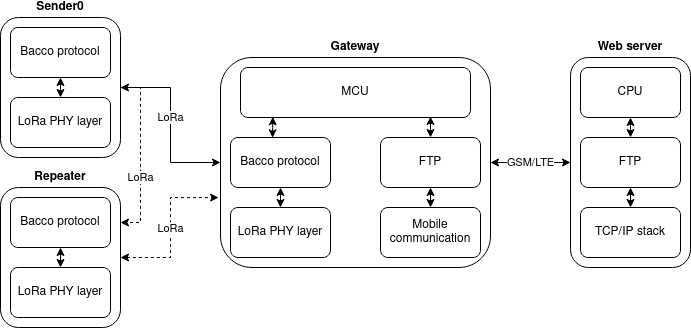
\includegraphics[width=1.0\textwidth]{uml/network_stack.png}
    \caption{Schematic representation of the used protocols}
    \label{network stack img}
\end{figure}

\section{Topology}
The network has a star-of-stars topology, in which the first level is occupied by the Web server and the
Gateways, wherease the second level contains the Gateways, the Repeaters and the Senders. \footnote{The use of Repeaters where
physical obstacles compromise the integrity of the signals is of very high
relevance in agricultural contexts, since natural barriers such as hills can easily block \gls{VHF} radio signals.}
Figure \ref{network topology img} shows the type of devices that are involved and their communication schema. \\
The structure is equivalent to a tree, hence we can define a hierarchy of nodes. The root node is the central web server
and its children nodes are the gateways. The gateways themselves are parents of either a repeater or a sender node,
which correspond to the leaves of the tree.

\begin{figure}[ht]
    \centering
    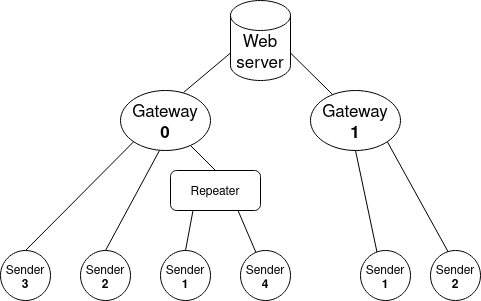
\includegraphics[width=350pt]{uml/network_topology.png}
    \caption{Network topology}
    \label{network topology img}
\end{figure}

\section{Addressing}
The addressing scheme follows from the hierarchical structure of the network.\\
A first description of the addressing algorithm is given in the case where there's a fixed number of nodes connected to the
network. Later the procedure will be extended in order to achieve the addition or removal of nodes from the network.

\subsection{Static addressing}
In order to uniquely identify each node in a static network represented as a tree, we can apply the following procedure:
\begin{itemize}
    \item{May $T$ be a tree and may $r$ be its root node}
    \item{May $\{T_{i}\}$ be a forest of substrees with cardinality of $I$, where $T_{i}$ is a subtree rooted in the child node
        $i$ of $r$, and $I$ is equal to the degree of $r$ }
    \item{For each node $i$, assing an identifier to it, that's unique among the other $i$s. In particular the integers
        contained in the interval $\[1,I\]$ will be used to represent each node}
    \item{RECURSIVELY}
    \item{CONCATENATE FROM ROOT TO NODE AND I HAVE THE ID}
\end{itemize}

address combined with the address of its parent node.
each Gateway is responsible of the addressing of its sender nodes. On the contrary Gateway nodes are manually assigned a
unique ID based on their physical location.
